\let\negmpace\undefined
\let\negthickspace\undefined
\documentclass[journal]{IEEEtran}
\usepackage[a5paper, margin=10mm, onecolumn]{geometry}
%\usepackage{lmodern} % Ensure lmodern is loaded for pdflatex
\usepackage{tfrupee} % Include tfrupee package
\setlength{\headheight}{1cm} % Set the height of the header box
\setlength{\headsep}{0mm}     % Set the distance between the header box and the top of the text
\usepackage{xparse}
\usepackage{gvv-book}
\usepackage{gvv}
\usepackage{cite}
\usepackage{amsmath,amssymb,amsfonts,amsthm}
\usepackage{algorithmic}
\usepackage{graphicx}
\usepackage{textcomp}
\usepackage{xcolor}
\usepackage{txfonts}
\usepackage{listings}
\usepackage{enumitem}
\usepackage{mathtools}
\usepackage{gensymb}
\usepackage{comment}
\usepackage[breaklinks=true]{hyperref}
\usepackage{tkz-euclide} 
\usepackage{listings}
% \usepackage{gvv}                                        
\def\inputGnumericTable{}                                 
\usepackage[latin1]{inputenc}                                
\usepackage{color}                                            
\usepackage{array}                                            
\usepackage{longtable}                                       
\usepackage{calc}                                             
\usepackage{multirow}                                         
\usepackage{hhline}                                           
\usepackage{ifthen}                                           
\usepackage{lscape}
\renewcommand{\thefigure}{\theenumi}
\renewcommand{\thetable}{\theenumi}
\setlength{\intextsep}{10pt} % Space between text and floats
\numberwithin{equation}{enumi}
\numberwithin{figure}{enumi}
\renewcommand{\thetable}{\theenumi}
\begin{document}
\bibliographystyle{IEEEtran}
\title{Question-10.4.2.1.2}
\author{EE24BTECH11038 - MALAKALA BALA SUBRAHMANYA ARAVIND}
% \maketitle
% \newpage
% \bigskip
{\let\newpage\relax\maketitle}
\textbf{Question}:
Find the roots of the equation $2x^2+x-6=0$\\
\solution \\
We can solve the above equation using fixed point iterations. First we separate $x$, from the above equation and make an update equation of the below sort.
\begin{align}
	x = g\brak{x} \implies x_{n+1} = g\brak{x_n}
\end{align}
Applying the above update equation on our equation, we get
\begin{align}
    x_{n+1}=6-2x_n^2\\
\end{align}
Now we take an initial value $x_0$ and iterate the above update equation. But we realize that the updated values always approach infinity for any initial value. \\
Thus we will alternatively use Newton's Method for solving equations.
\begin{align}
	x_{n+1} = x_n - \frac{f\brak{x_n}}{f^{\prime}\brak{x_n}} 
\end{align}
Where we define $f\brak{x}$ as, 
\begin{align}
	f\brak{x} = 2x^2+x-6 \\
	f^{\prime}\brak{x} = 4x+1
\end{align}
Thus, the new update equation is, 
\begin{align}
	x_{n+1} = x_n - \frac{2x_n^2+x_n-6}{4x_n+1 } 
\end{align}
Taking an initial guess of $x_0=-4$ we can see that $x_n$ converges at the 3rd iteration with x as
\begin{align}
    x=-2
\end{align}
Taking an initial guess of $x_0=1$ we can see that $x_n$ converges at the 3rd iteration with x as
\begin{align}
    x=\frac{3}{2}
\end{align}


\textbf{CODING LOGIC FOR FINDING EIGENVALUES :-}\\


The quadratic equation 
\begin{align}
2x^2+x-6=0
\end{align}
is rewritten in matrix form:
\begin{align}
\text{Matrix} =
\myvec{0 & -\frac{c}{a} \\
1 & -\frac{b}{a}
}
\end{align}

\begin{align}
a = 2, \quad b=1, \quad c = -6.
\end{align}

Substituting the values of $a,b$ and $c$, the matrix becomes:\\
Let
\begin{align}
\text{A} =
\myvec{0 & 3 \\
1 & -\frac{1}{2}
}
\end{align}




\textbf{QR-Algorithm}\\
The QR method is an iterative algorithm used to compute the eigenvalues of a square matrix $A$. The algorithm works as follows:
\begin{enumerate}
\item Initialization \\
Let $A_0 = A $, where $A$ is the given matrix.

\item QR Decomposition \\
For each iteration $ k = 0, 1, 2, \dots $:
\begin{enumerate}
    \item Compute the QR decomposition of \( A_k \), such that:
    \begin{align}
    A_k = Q_k R_k
    \end{align}
    where:
    \begin{enumerate}
        \item $Q_k $ is an orthogonal matrix ($ Q_k^\top Q_k = I $).
        \item $ R_k $ is an upper triangular matrix.
    \end{enumerate}
    The decomposition ensures $ A_k = Q_k R_k $.

    \item Form the next matrix \( A_{k+1} \) as:
    \begin{align}
    A_{k+1} = R_k Q_k
    \end{align}
\end{enumerate}

\item Convergence\\
Repeat Step 2 until $ A_k $ converges to an upper triangular matrix $ T $. The diagonal entries of $T$ are the eigenvalues of $A$.\\
\item The eigenvalues of matrix will be the roots of the equation.
\begin{figure}[h!]
	\centering
	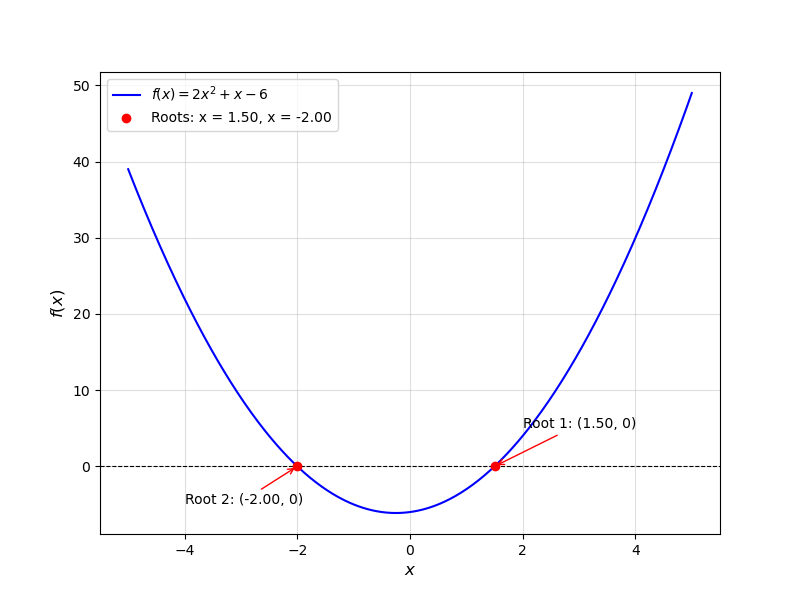
\includegraphics[width=\columnwidth]{figs/Figure_1.png}
	\label{stemplot}
\end{figure}

\end{enumerate}
\end{document}
